\section{Projections for LHC neutrino structure functions}
\label{sec:dis_pseudodata}

We begin by describing the procedure adopted to generate
projections for LHC neutrino DIS structure functions, including
the models for the expected systematic uncertainties associated
to the various experiments.


\subsection{Recap of DIS kinematics}

The double-differential cross-section for neutrino-nucleus scattering
can be decomposed
in terms of three independent structure functions $F_i^{\nu A}(x,Q^2)$ with $i=1,2,3$.
%
Focusing on the charged-current (CC) scattering case, mediated
by the exchange of a $W^+$ weak boson, the differential
 cross section reads
\be
\label{eq:neutrino_DIS_xsec}
\frac{d^2\sigma^{\nu A}(x,Q^2,y)}{dxdy} =  \frac{G_F^2s/2\pi}{\lp 1+Q^2/m_W^2\rp^2}\lc (1-y)F^{\nu A}_2(x,Q^2) + y^2xF^{\nu A}_1(x,Q^2) + y\lp 1-\frac{y}{2}\rp xF^{\nu A}_3(x,Q^2)\rc  \, ,
\ee
where $s=2m_N E_\nu$ is the neutrino-nucleon center of mass energy squared, $m_N$ is the nucleon mass,
$E_\nu$ is the incoming neutrino energy,
and the inelasticity $y$ is defined as $y=Q^2/(2x m_n E_{\nu})$.
%
For the time being we are neglecting target mass 
corrections.
%
An analogous expression holds for  antineutrino 
scattering, mediated
by the exchange of a $W^-$ weak boson, with the only difference being a sign change
in front of the parity-violating structure function $xF_3$,
\be
\label{eq:antineutrino_DIS_xsec}
\frac{d^2\sigma^{\bar{\nu} A}(x,Q^2,y)}{dxdy} =  \frac{G_F^2s/2\pi}{\lp 1+Q^2/m_W^2\rp^2}\lc (1-y)F^{\bar{\nu} A}_2(x,Q^2) + y^2xF^{\bar{\nu} A}_1(x,Q^2) - y\lp 1-\frac{y}{2}\rp xF^{\bar{\nu} A}_3(x,Q^2)\rc  \, .
\ee
While the differential cross-section depends on three kinematic variables, $(x,Q^2,y)$,
the structure functions themselves depend only on $x$ and $Q^2$.
%
Furthermore, both the cross-section and the structure functions depend
on the atomic mass number $A$ of the target nucleus via nuclear modifications of the free-nucleon
structure functions.

Alternatively, Eq.~(\ref{eq:neutrino_DIS_xsec}) can be expressed in terms
of the longitudinal structure function  $F_L^{\nu A}(x,Q^2)$ defined
by $F_L = F_2-2xF_1$, leading to
\be
\label{eq:neutrino_DIS_xsec_FL}
\frac{d^2\sigma^{\nu A}(x,Q^2,y)}{dxdy} =  \frac{G_F^2s/4\pi}{\lp 1+Q^2/m_W^2\rp^2}\lc Y_+F^{\nu A}_2(x,Q^2) - y^2F^{\nu A}_L(x,Q^2) +Y_- xF^{\nu A}_3(x,Q^2)\rc  \, ,
\ee
where $Y_\pm = 1 \pm (1-y)^2$ and with a counterpart expression for anti-neutrino scattering,
\be
\label{eq:antineutrino_DIS_xsec_FL}
\frac{d^2\sigma^{\bar{\nu} A}(x,Q^2,y)}{dxdy} =  \frac{G_F^2s/4\pi}{\lp 1+Q^2/m_W^2\rp^2}\lc Y_+F^{\bar{\nu} A}_2(x,Q^2) - y^2F^{\bar{\nu} A}_L(x,Q^2) -Y_- xF^{\bar{\nu} A}_3(x,Q^2)\rc  \, ,
\ee
%
Expressing the differential cross-section as in Eq.~(\ref{eq:neutrino_DIS_xsec_FL}) is advantageous
because in the parton model (and in perturbative QCD at leading order) the longitudinal
structure function vanishes, $F_L^{\nu A}(x,Q^2)=0$.
%
The combination of neutrino and antineutrino measurements makes possible disentangling
the different structure functions, for example the cross-section difference
\be
\label{eq:neutrino_DIS_xsec_FL_diff}
\frac{d^2\sigma^{\nu A}(x,Q^2,y)}{dxdy} - \frac{d^2\sigma^{\bar{\nu} A}(x,Q^2,y)}{dxdy}=  \frac{G_F^2s Y_-}
{4\pi \lp 1+Q^2/m_W^2\rp^2}\lc    xF^{\nu A}_3(x,Q^2)+  xF^{\bar{\nu} A}_3(x,Q^2)\rc \, ,
\ee
is proportional to the parity-violating structure function $xF_3$ averaged over neutrinos
and antineutrinos.

When both the momentum transfer squared $Q^2$
and the  hadronic final-state
invariant mass $W$ given by
\be
W^2 = m_N^2 + Q^2 \frac{(1-x)}{x} \, ,
\ee
are large enough, $Q^2 \gsim {\rm few~GeV}^2$ and $W \gsim 2$ GeV
respectively, we find ourselves in the
deep-inelastic scattering region where
structure functions can be evaluated in perturbative QCD in terms of a factorised
convolution of process-dependent partonic scattering cross-sections and
of process-independent parton distribution functions,
\be
\label{eq:sfs_pqcd}
 F^{\nu A}_i(x,Q^2) = \sum_{j=q,\bar{q},g}\int_x^1 \frac{dz}{z}\, C_{i,j}^{\nu N}(z,\alpha_s(Q^2))f^{(A)}_j\lp \frac{x}{z},Q^2\rp \, , \quad i = 2,3,L \, ,
 \ee
 where $j$ is an index that runs over all possible partonic initial states
 and $C_{i,j}^{\nu N}$ is the process-dependent (but target-independent) coefficient function.
 %
 The latter can be expressed  as a series expansion in powers of the strong
 coupling $\alpha_s(Q^2)$,
 \be
 \label{eq:coeff_fun_expansion}
 C_{i,j}^{\nu N}(z,\alpha_s(Q^2)) = \sum_{k=0}^m \lp \alpha_s(Q^2) \rp^{k} C_{i,j}^{\nu N(k)}(z) \, .
 \ee
 The leading-order ($k=0$)  term is independent of $\alpha_s$ since the Born scattering
 is mediated by the weak interaction.
 %
 At leading order and considering a proton target, $n_f=4$ active quark flavours,
 neglecting charm mass effects and assuming a diagonal CKM matrix,
 we can express the $F_2^{\nu p}$ and $xF_3^{\nu p}$ structure functions as
 follows
 \bea
 F_2^{\nu p}(x,Q^2) &=& 2x\lp f_{\bar{u}} + f_{d} + f_{s} + f_{\bar{c}} \rp(x,Q^2) \, , \nonumber  \\
 F_2^{\bar{\nu} p}(x,Q^2) &=& 2x\lp f_u + f_{\bar{d}} + f_{\bar{s}} + f_c \rp(x,Q^2) \, , \label{eq:neutrinoSFs} \\
 xF_3^{\nu p}(x,Q^2) &=& 2x\lp -f_{\bar{u}} + f_d +f_s - f_{\bar{c}}\rp(x,Q^2)  \, , \nonumber\\
 xF_3^{\bar{\nu} p}(x,Q^2) &=& 2x\lp f_u - f_{\bar{d}} -f_{\bar{s}} + f_{c}\rp(x,Q^2) \, . \nonumber
 \eea
 The corresponding expressions for a neutron target and or isoscalar target can be obtained
 from isospin symmetry, for instance the LO structure functions for
 neutrino-neutron scattering are
 \bea
 F_2^{\nu n}(x,Q^2) &=& 2x\lp f_{\bar{d}} + f_{u} + f_{s} + f_{\bar{c}} \rp(x,Q^2) \, , \nonumber  \\
 F_2^{\bar{\nu} n}(x,Q^2) &=& 2x\lp f_d + f_{\bar{u}} + f_{\bar{s}} + f_c \rp(x,Q^2) \, , \label{eq:antineutrinoSFs} \\
 xF_3^{\nu n}(x,Q^2) &=& 2x\lp -f_{\bar{d}} + f_u +f_s - f_{\bar{c}}\rp(x,Q^2)  \, , \nonumber\\
 xF_3^{\bar{\nu} n}(x,Q^2) &=& 2x\lp f_d - f_{\bar{u}} -f_{\bar{s}} + f_{c}\rp(x,Q^2) \, . \nonumber
 \eea
 

\subsection{DIS pseudo-data generation}
\label{sec:pseudo-data_generation}

The first goal is to produce projections
for DIS pseudo-data at the FPF based on
some idealised detector concepts and
some initial choice of neutrino fluxes
e.g.~\cite{Kling:2021gos}.
%
This requires a knowledge of the detector geometry
and material, as well as of the double-differential
neutrino interaction cross-section. 
%
Since we aim to produce pseudo-data binned in $(x,Q^2)$,
for each simulated event we need to determine the 
final-state kinematics. 

Specifically, we would like to evaluate the
number of charged-current neutrino interaction events
within the detector volume in different bins
of the incoming neutrino energy $E_\nu$, the Bjorken
variable $x$ and the momentum transfer square $Q^2$,
\begin{equation}
    N_{\rm ev}(E_\nu, x, Q^2) \, ,
\end{equation}
for some binning in these three kinematic variables.
%
This can be evaluated as
\begin{equation}
\label{eq:nev_v1}
    N_{\rm ev}(E_\nu, x, Q^2) \propto \int_{\rm bin}\int_{\rm det}  \frac{d^2\sigma^{\nu A}(x,Q^2,y)}{dxdy} \mathcal{L}_{\nu}(E_{\nu}) \, ,
\end{equation}
where $\mathcal{L}(E_{\nu}) $ is the incoming neutrino
luminosity which accounts for the detector geometry
and material density. 
%
Eq.~(\ref{eq:nev_v1}) can be integrated to
determine the actual number of events within
the bin boundaries.

We start with a perfect detector.


For bins in $x,Q^2,E_{\nu}$, we start with the \href{https://github.com/juanrojochacon/FPF-WG1/blob/main/results/diff_xsecs_a1.txt}{differential cross section},$\frac{d^2\sigma(x,Q^2,E_{\nu}}{dxdQ^2})$ [pb GeV$^{-2}$] as output from {\tt YADISM} and convolve with the \href{https://github.com/KlingFelix/FastNeutrinoFluxSimulation/tree/main/Fluxes}{neutrino flux}, $\frac{dN_{\nu}}{dE_{\nu}}$. So for a detector with $n_T$ nuclear target density and $L_T$ length, we calculate the event rate per bin as

\begin{equation}
    N_{\rm ev}/{\rm bin} = n_T L_T\int_{Q^2_{min}}^{Q^2_{max}}\int_{x_{min}}^{x_{max}}\int_{E_{\nu,min}}^{E_{\nu , max}} \frac{dN_{\nu}}{dE_{\nu}}\left(\frac{d^2\sigma(x,Q^2,E_{\nu})}{dxdQ^2}\right) dQ^2 dx dE_{\nu}.
\end{equation}

Using a MC integration, we can calculate $N_{\rm ev}/{\rm bin}$ by sampling $N$ points in $x,Q^2,E_{\nu}$ space such that $0< y = \frac{Q^2}{2m_N E_{\nu }x} < 1$ and integrating over the bin.

\begin{equation}
    N_{\rm ev}/{\rm bin} \approx n_T L_T \frac{(Q^2_{max}-Q^2_{min})(x_{max}-x_{min})(E_{\nu ,max}-E_{\nu ,min})}{N}\times \sum_i^N f(x_i,Q^2_i,E_{\nu ,i})
    \label{MCintegration}
\end{equation}

where $f(x_i,Q^2_i,E_{\nu ,i}) = \frac{dN_{\nu}}{dE_{\nu,i}}\left(\frac{d^2\sigma(x_i,Q^2_i,E_{\nu,i})}{dxdQ^2}\right)$. 

The statistical uncertainty for each bin is then defined by a Gaussian distribution with fractional uncertainty $1/\sqrt{N{\rm ev}/{\rm bin}}$, i.e. $\delta N_{\rm ev}/{\rm bin} = \sqrt{N_{\rm ev}} /{\rm bin}$


  Following this prescription, we can produce plots which characterize the event rate for a particular neutrino species at a particular experiment. 

Results for FASER$\nu$2 can be found \href{https://github.com/juanrojochacon/FPF-WG1/tree/main/results}{here}. The .txt files will display which neutrino species was considered, and also compile experimental geometries and target details in the header. In the sub-folder \href{https://github.com/juanrojochacon/FPF-WG1/tree/main/results/Summaries}{summaries}, plots can be found which show the event rate in $x,Q^2$ space, integrating over the entire neutrino spectrum. The event rate for muon neutrinos at FASER$\nu$2 is shown in Fig~\ref{fig:fasernu2_muon}.

\begin{figure}[h]
    \centering
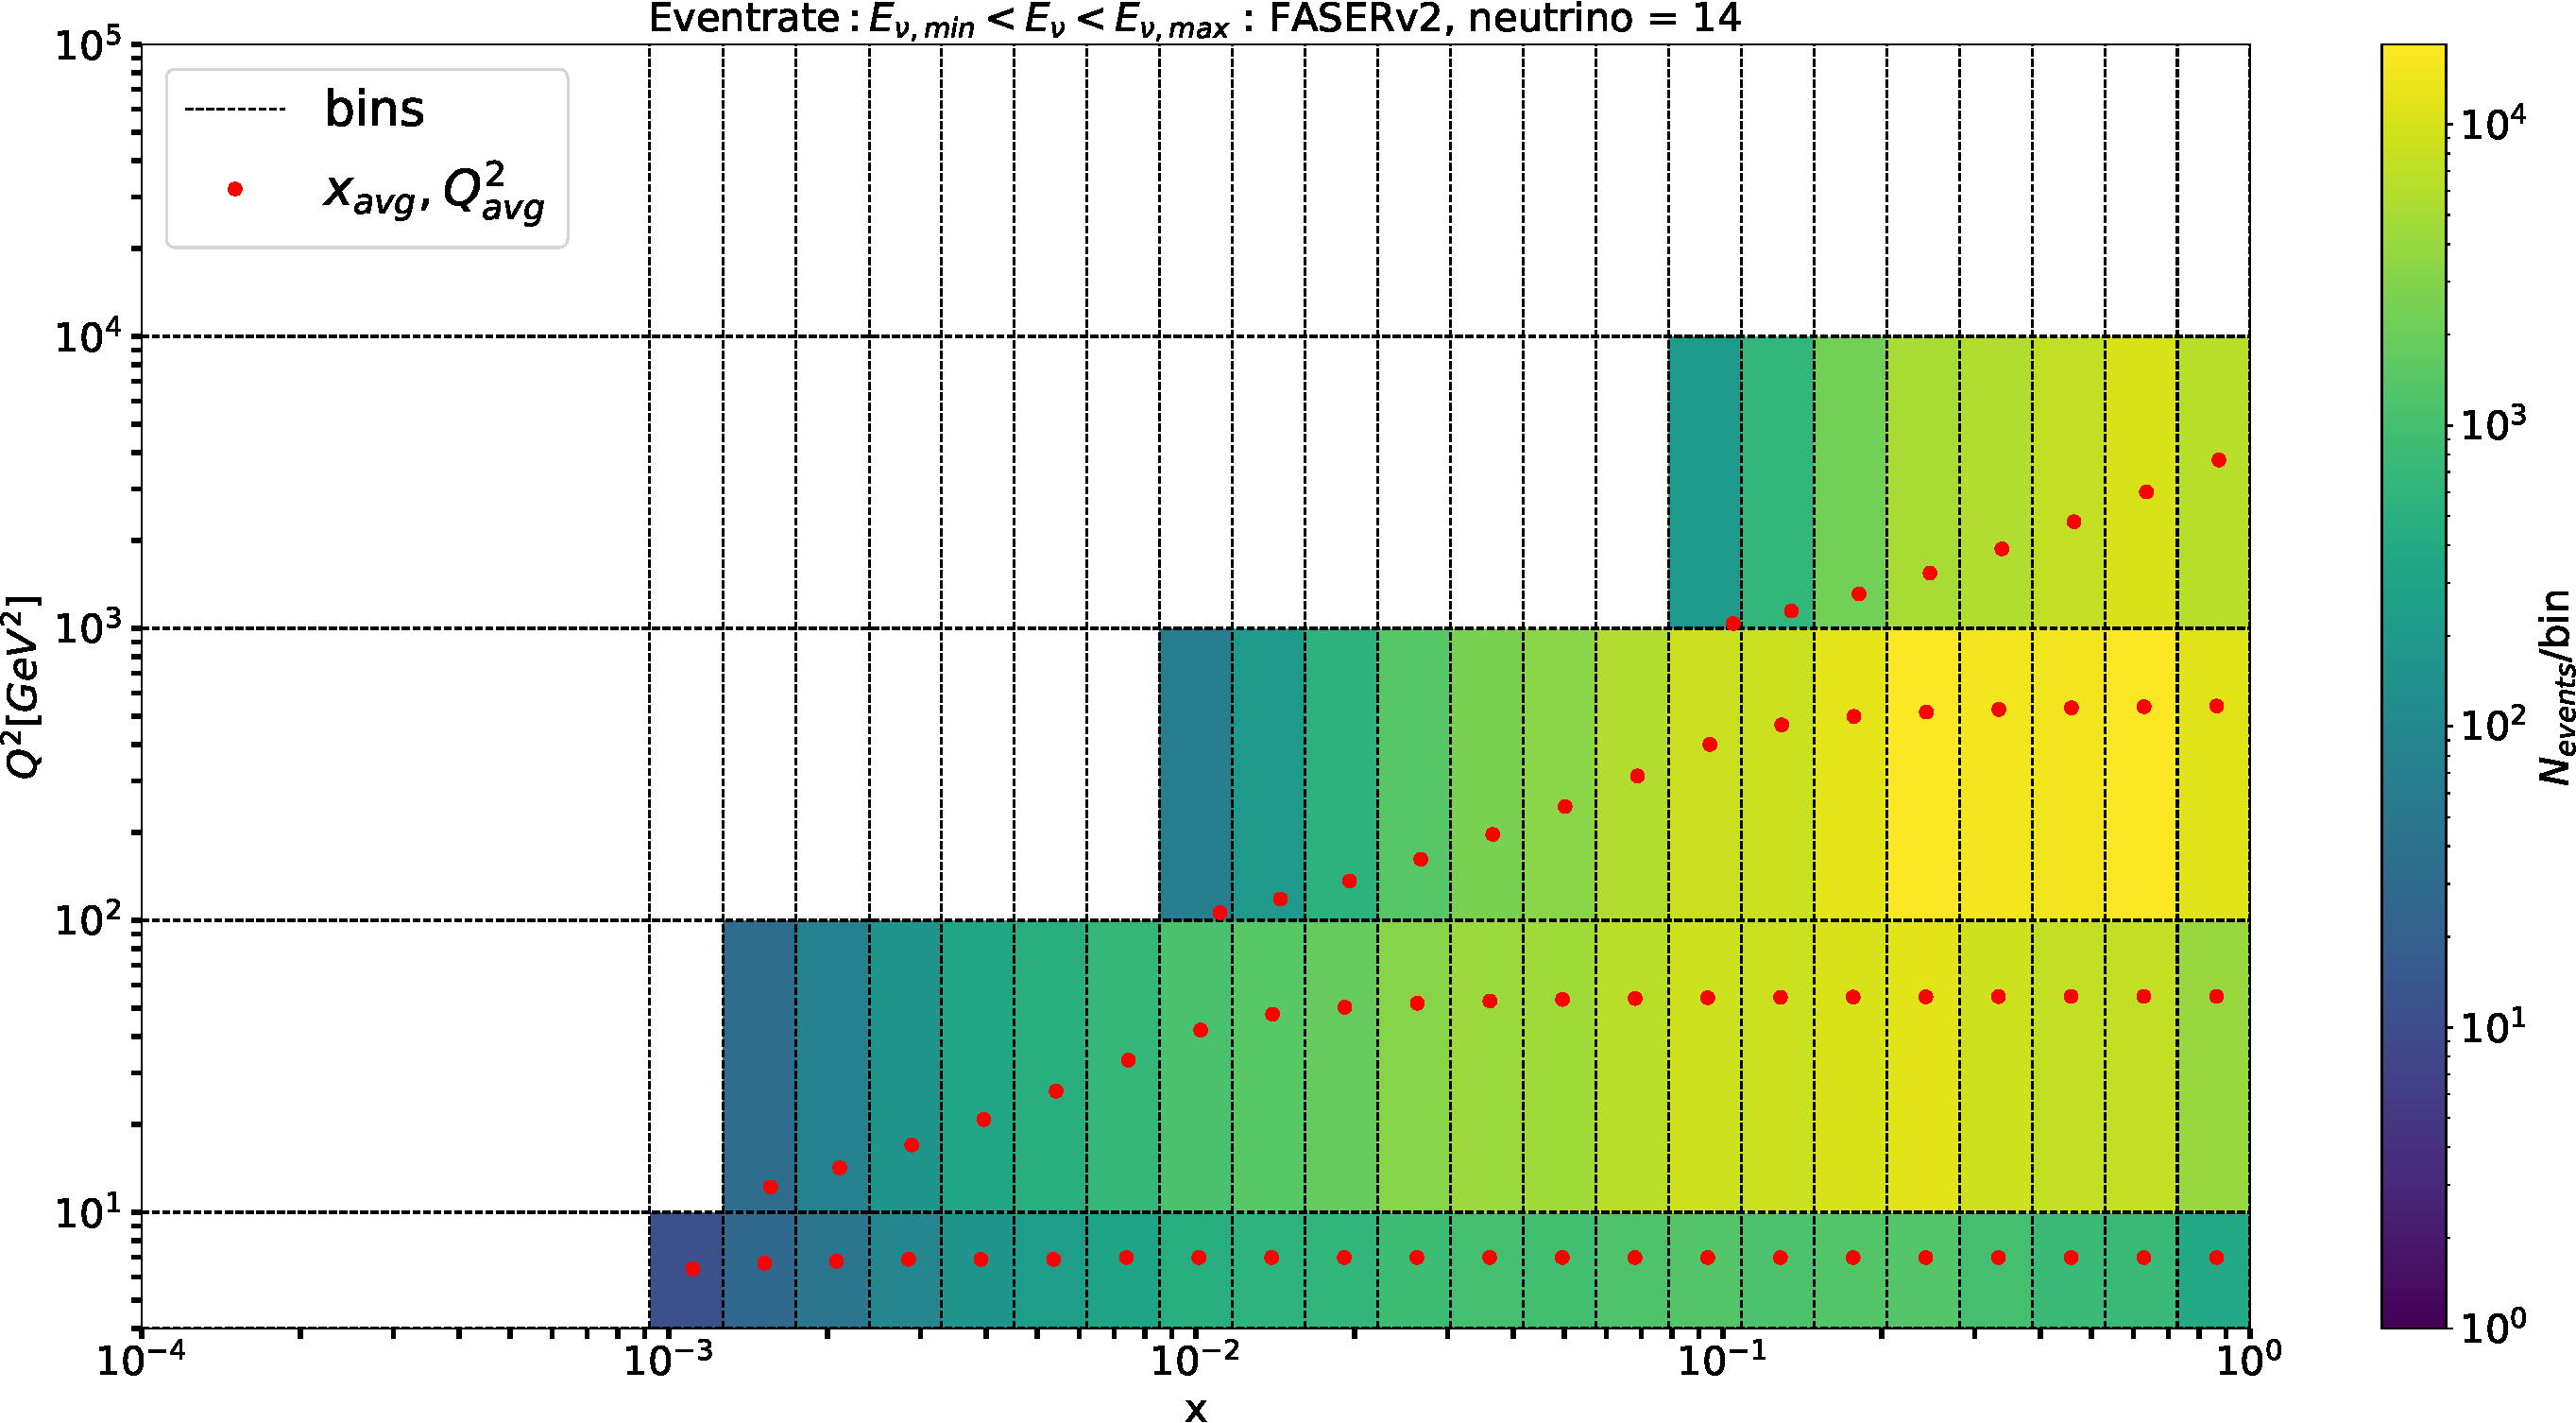
\includegraphics[width=1\textwidth]{plots/Nevent_FASERv2_14.pdf}
    \caption{Event rate per bin for muon neutrinos at FASER$\nu$2. Bins are denoted by dashed grid, and the red dot indicates the weighted average of $x,Q^2$ points in each bin. The total number of muon neutrino events calculated is $\approx2.6\times 10^5$. Note that bins were chosen somewhat arbitrarily, and can be iterated to improve PDF fits }
    \label{fig:fasernu2_muon}
\end{figure}

\subsection{Systematic Effects on Pseudodata}
We now wish to understand the impact of systematic uncertainties on the event rate in $(x,Q^2,E_{\nu})$ space. For each experiment, the observables $E_{l},E_{h},\theta$ are related to $(x,Q^2,E_{\nu})$ by 

\begin{align}
E_{\nu} = E_l + E_h \nonumber \\
Q^2 = 4E_lE_{\nu}\sin^2{\theta/2} \nonumber \\
x = \frac{Q^2}{2m_N(E_{\nu} - E_l)}.
\end{align}

We wish to sample over the space of observables, $(E_{l},E_{h},\theta)$, perform  cuts based on detector performance, calculate the event rates, and then smear this sampling according to experimental uncertainties to estimate the uncertainty on the event rate. 

Taking FASER${\nu}$2 as an example, we can write the experimental cuts and uncertainties as 

\begin{align}
100 < E_l < E_{\nu,{\rm max}} , \delta E_l = 30\% \nonumber \\
100 < E_h < E_{\nu,{\rm max}} , \delta E_h = 50\% \nonumber \\
0 < \theta < \tan^{-1}(0.5) , \delta\theta = 1~{\rm mrad}
\label{fasernu2systematic_errors}
\end{align}

We first generate a MC dataset, $D_0$, over this space with $N = 10^7$ samples and calculate $x,Q^2,E_{\nu}$ for each event, removing samples with $y > 1$. We then integrate according to Eq. \ref{MCintegration} to produce a distribution of events with bins in $x,Q^2,E_{\nu}$. We then smear each sample according to a Gaussian distribution with widths given by Eq.~\ref{fasernu2systematic_errors} to produce a new data set $D_i$ and repeat to produce $M = 10$ event distributions($M>10$ can later be used, but $M = 10$ appears to be stable). For each bin we take the standard deviation to produce the systematic errors per bin (denoted as "N\textunderscore sys\textunderscore errs" in files named "binned\textunderscore sys-events... .txt" \href{https://github.com/juanrojochacon/FPF-WG1/tree/main/results}{here}). 

For FASER${\nu}$2, the systematic errors typically dominate over statistical errors, at about $10\%$. 

\begin{figure}[h]
    \centering
    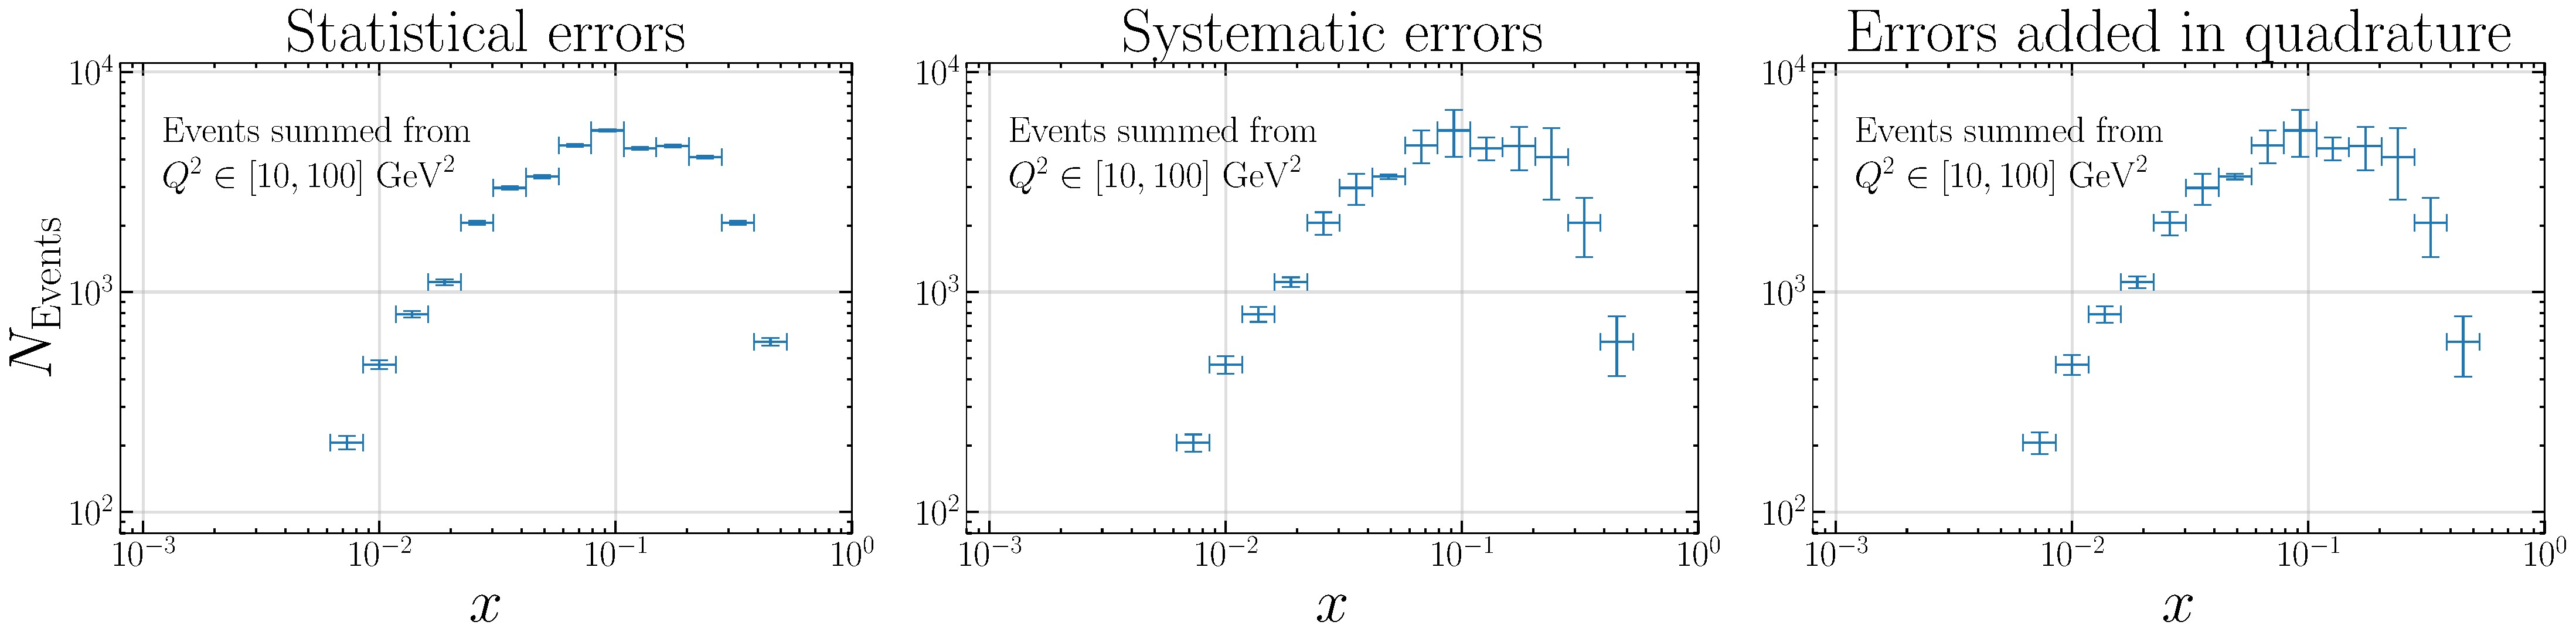
\includegraphics[width = 1\textwidth]{plots/error_plot_FASERv2_14.pdf}
    \caption{Event rates with error bars at FASER$\nu$2 for $\nu_{\mu} N \rightarrow \mu^- X$} summed over $Q^2$. The error bars along the x-axis showing the width of the $x$-bins, and are not showing any type of error.
    \label{fig:my_label}
\end{figure}

\subsection{Experimental acceptance performance} 

\paragraph{AdvSND} 
\begin{itemize}
    \item The detectors will be able to track muons that have energy greater
    than $20~\rm{GeV}$ (the values for the other charged leptons remain to be
    determined) with an acceptance angle of 100 mrad for the muons and 
    500 mrad for the both electrons and tau.
    \item In addition, the information on the charge of the outgoing leptons
    can also be accessed.
    \item It should also be possible to reconstruct the hadronic final states
    by measuring the total energy.
\end{itemize}

\paragraph{FLArE}
\begin{itemize}
    \item The detectors will be able to detect electrons with energy up to
    $1~\rm{TeV}$ and an acceptance angel as high as 0.5 rad. For the muons,
    the detectors will only be able to track them up to $1.5~\rm{GeV}$ with
    a scattering angle reaching up to 0.4 mrad. The reconstruction of the
    tau's angle and energy instead will be very difficult. However, it might
    be possible to find the vertex of a particular tau decay if fine position
    resolution is achieved.
    \item With the current baseline design of the detector, it will not be
    possible to access the information on the sign of the charged leptons.
    \item It should also be possible to reconstruct the hadronic final
    states but the reconstruction efficiency and particles will depend on
    the type of particles. It is expected that the final states hadrons will
    be dominated by pions, protons, and neutrons.
    \item Regarding the systematic errors on the charged lepton energy and
    scattering angle, it is expected to get $5\%$ energy resolution for
    electrons and about 15 mrad in angular resolution. Due to the large
    missing energy in the detector, $30\%$ energy resolution is probably
    achievable for muons with about 5 mrad angular resolution.
\end{itemize}
